\documentclass[tikz,border=12pt]{standalone}
\usepackage{amsmath,amssymb}
\usetikzlibrary{calc,arrows.meta}

\begin{document}
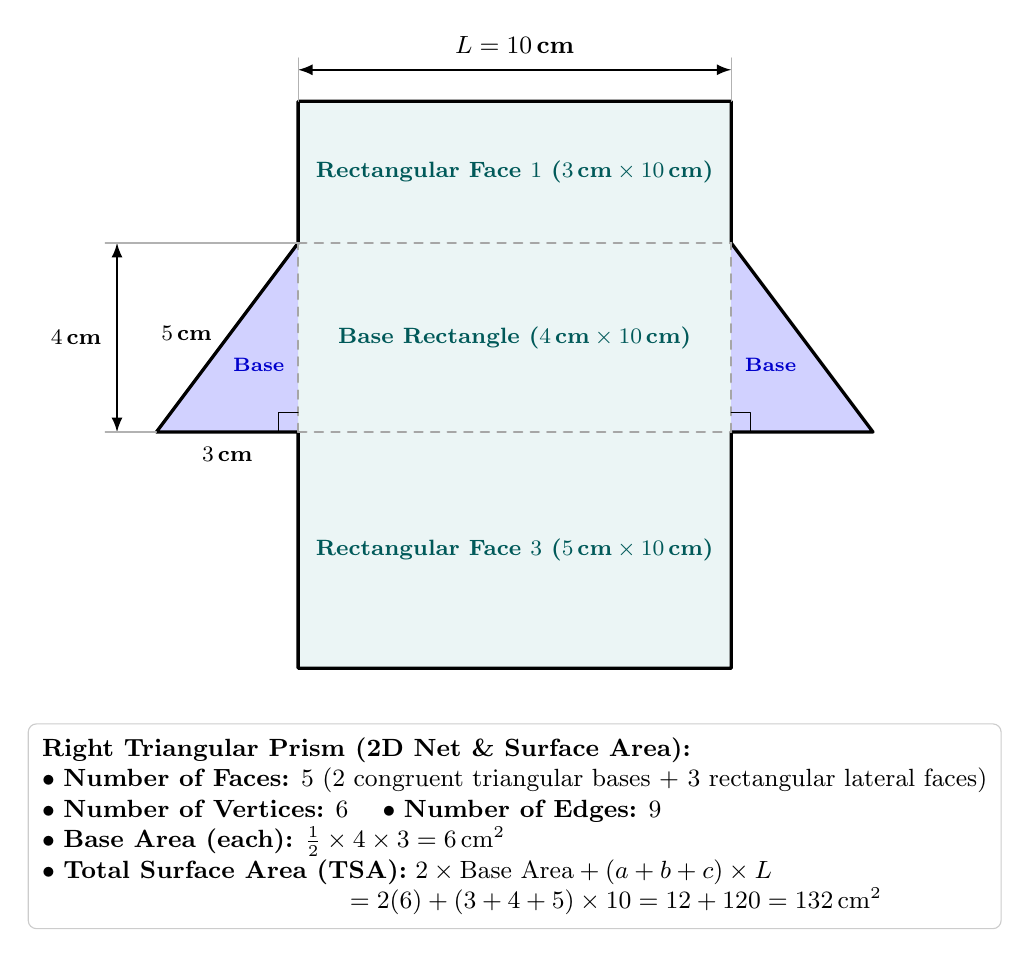
\begin{tikzpicture}[>=latex, line cap=round, line join=round]

  % Dimensions (3-4-5 right triangle, length L = 5.5)
  % Scale: a = 1.8 (represents 3 cm), b = 2.4 (represents 4 cm), c = 3.0 (represents 5 cm), L = 5.5 (represents 10 cm)
  \def\a{1.8}
  \def\b{2.4}
  \def\c{3.0}
  \def\L{5.5}

  % Shading of faces
  % Lateral rectangular faces (teal!8)
  \fill[teal!8] (0, -\c) rectangle (\L, \b + \a);
  % Triangular base flaps (blue!18)
  \fill[blue!18] (0, 0) -- (-\a, 0) -- (0, \b) -- cycle;
  \fill[blue!18] (\L, 0) -- (\L + \a, 0) -- (\L, \b) -- cycle;

  % Outer boundary (solid thick lines)
  \draw[very thick] (0, \b + \a) -- (\L, \b + \a) -- (\L, \b) -- (\L + \a, 0) -- (\L, 0) -- (\L, -\c) -- (0, -\c) -- (0, 0) -- (-\a, 0) -- (0, \b) -- cycle;

  % Interior fold lines (dashed)
  \draw[thick, dashed, gray!70] (0, \b) -- (\L, \b);
  \draw[thick, dashed, gray!70] (0, 0) -- (\L, 0);
  \draw[thick, dashed, gray!70] (0, 0) -- (0, \b);
  \draw[thick, dashed, gray!70] (\L, 0) -- (\L, \b);

  % Right angle symbols on triangular flaps
  \draw[thin] (0, 0.25) -- (-0.25, 0.25) -- (-0.25, 0);
  \draw[thin] (\L, 0.25) -- (\L + 0.25, 0.25) -- (\L + 0.25, 0);

  % Face labels inside regions
  \node[font=\footnotesize\bfseries, teal!70!black] at (\L/2, \b + \a/2) {Rectangular Face $1$ ($3\,\text{cm} \times 10\,\text{cm}$)};
  \node[font=\footnotesize\bfseries, teal!70!black] at (\L/2, \b/2) {Base Rectangle ($4\,\text{cm} \times 10\,\text{cm}$)};
  \node[font=\footnotesize\bfseries, teal!70!black] at (\L/2, -\c/2) {Rectangular Face $3$ ($5\,\text{cm} \times 10\,\text{cm}$)};
  \node[font=\scriptsize\bfseries, blue!80!black] at (-0.5, 0.85) {Base};
  \node[font=\scriptsize\bfseries, blue!80!black] at (\L + 0.5, 0.85) {Base};

  % Dimension callouts
  % Length of prism (top dimension)
  \draw[thick, <->] (0, \b + \a + 0.4) -- (\L, \b + \a + 0.4) node[midway, above=2pt, font=\small\bfseries] {$L = 10\,\text{cm}$};
  \draw[thin, gray!60] (0, \b + \a) -- (0, \b + \a + 0.55);
  \draw[thin, gray!60] (\L, \b + \a) -- (\L, \b + \a + 0.55);

  % Side lengths on left triangular flap
  \node[below=2pt, font=\footnotesize\bfseries] at (-\a/2, 0) {$3\,\text{cm}$};
  \node[left=3pt, font=\footnotesize\bfseries, fill=white, inner sep=1pt] at (-0.95, 1.25) {$5\,\text{cm}$};

  % Central rectangle width
  \draw[thick, <->] (-\a - 0.5, 0) -- (-\a - 0.5, \b) node[midway, left=2pt, font=\footnotesize\bfseries] {$4\,\text{cm}$};
  \draw[thin, gray!60] (-\a, 0) -- (-\a - 0.65, 0);
  \draw[thin, gray!60] (0, \b) -- (-\a - 0.65, \b);

  % Formula Card below
  \node[align=left, font=\small, fill=white, inner sep=5pt, draw=gray!40, rounded corners=3pt, anchor=north] at (\L/2, -\c - 0.7) {
    \textbf{Right Triangular Prism (2D Net \& Surface Area):}\\
    $\bullet$ \textbf{Number of Faces:} 5 (2 congruent triangular bases + 3 rectangular lateral faces)\\
    $\bullet$ \textbf{Number of Vertices:} 6 \quad $\bullet$ \textbf{Number of Edges:} 9\\
    $\bullet$ \textbf{Base Area (each):} $\frac{1}{2} \times 4 \times 3 = 6\,\text{cm}^2$\\
    $\bullet$ \textbf{Total Surface Area (TSA):} $2 \times \text{Base Area} + (a + b + c) \times L$\\
    \hspace*{38mm} $= 2(6) + (3 + 4 + 5) \times 10 = 12 + 120 = 132\,\text{cm}^2$
  };

\end{tikzpicture}
\end{document}
